% ----------------------------------------------------------
% Introdução (exemplo de capítulo sem numeração, mas presente no Sumário)
% ----------------------------------------------------------
\chapter[Revisão Bibliográfica]{Revisão Bibliográfica}
%$\addcontentsline{toc}{chapter}{Introdução}
% ----------------------------------------------------------

A literatura sobre Receptores Ópticos \'e extensa e contempla os mais diversos aspectos sobre o tema, desde o entendimento do fenômeno físico, diferentes topologias e estrat\'egias para otimização de diferentes características do circuito, circuitos auxiliares necessários para a transferência de informação, e tamb\'em o layout do projeto. Este capítulo tem como objetivo contextualizar e fundamentar algumas discussões de capítulos posteriores, demonstrar alguns trabalhos previamente realizados na área, e dar uma perspectiva histórica sobre algumas tecnologias envolvidas.
\section{Histórico}
O interesse de extrair informações advindas do espectro eletromagn\'etico \'e a muito tempo de grande interesse para físicos e engenheiros. As suas aplicações são diversas, desde extrair cores para formar uma imagem at\'e extrair informação digital de acordo com um sinal luminoso modulado.
Em 1949, a primeira patente relacionada a um dispositivo semicondutor capaz de transformar informações luminosas em el\'etricas foi requisitada pela Bell Labs, sendo oficialmente aceita em 1951. Era o nascimento do fototransistor, um transistor bipolar especial que capta informação luminosa em sua base, gerando uma informação por forma de uma corrente el\'etrica em seu coletor e emissor \cite{Shive}.

Com invenção do fototransistor e fotodiodo, e o desenvolvimento de tecnologias de fabricação de semicondutores, se gerou uma intensa pesquisa na d\'ecada de 60, que culminou no desenvolvimento do CCD (\emph{Charge Coupled Device}) no início da d\'ecada de 70, sendo a tecnologia de Recepção Óptica mais utilizada at\'e a d\'ecada de 90 \cite{EstevaoCoelho, Andre}.

Em meados da d\'ecada de 70, o PPS (\emph{Passive Pixel Sensor}) foi desenvolvido, como alternativa aos dispositivos de imagem de tubo a vácuo \cite{Savvas}. Sua constituição se dá por uma matriz de fotodiodos, que convertem uma informação luminosa em el\'etrica, diretamente a um elemento processador de dados analógico, sem a utilização de um componente de amplificação.

Ainda na d\'ecada de 70, os primeiros trabalhos relacionados ao \emph{APS} foram desenvolvidos utilizando a tecnologia \emph{MOS} (\emph{Metal-Oxide-Semiconductor}) \cite{Peter}. O \emph{APS} \'e uma evolução direta do \emph{PPS} (\emph{Passive Pixel Sensor}), com a adição de um dispositivo amplificador \cite{EstevaoCoelho}. Amplificar o sinal permite uma maior precisão na aquisição dos dados, al\'em de permitir uma maior miniaturização do fotodiodo, o que leva a uma miniaturização de todo o sistema. Com a evolução da tecnologia CMOS (\emph{Complementary Metal-Oxide-Semiconductor}) na d\'ecada de 90, o \emph{APS} se tornou mais atraente, por ser facilmente integrado com outros componentes que utilizam-se da mesma tecnologia em um mesmo circuito integrado. O \emph{APS} vem desde então dominando o mercado de Recepção Óptica \cite{Andre, LidianeCampos}.

Amplificadores Operacionais s\~ao circuitos amplamente utilizados para o desenvolvimento de sistemas analógicos. Desde a década de 60, o desenvolvimento de circuitos de comunicação óptica exploram a utilização de amplificadores para captação de sinais ópticos, transmissão e regeneração de sinais. A utilização de amplificadores operacionais junto à fotodiodos, possibilitam a conversão de sinais de luz em elétricas, que pode ser então processado e utilizado para fins tanto analógicos quanto digitais. O circuito comumente utilizado no processo de captação óptica são variações do \emph{TIA}, tendo papel fundamental para a expansão tecnológica que vemos tendo desde então. \cite{ajoy, andrefontoura}.

\section{Fotodiodo}

O fotodiodo, ou fotodetector, \'e um componente optoeletrônico semicondutor que tem a função de captar um sinal eletromagn\'etico no ambiente, e então convertê-lo para uma corrente el\'etrica, chamada de corrente fotogerada, ou tamb\'em fotocorrente \cite{RazaviOpt}. A faixa de frequência do sinal que pode ser captado varia em cada projeto, mas dispositivos práticos se apresentam comumente em uma banda entre o ultravioleta e o infravermelho, o que possibilita o desenvolvimento de dispositivos dentro da faixa da luz visível \cite{LidianeCampos}.

Para o entendimento do funcionamento do fotodiodo, uma fundamentação quântica da luz deve ser utilizada, com foco principal na Teoria das Bandas e no entendimento do que são os Fótons.

\subsection{Física Quântica e Fotóns}
A Física Quântica nos diz que qualquer material apresenta níveis de energia possíveis dados de forma discreta (quantizada), ou seja, qualquer objeto do universo não pode ter qualquer nível de energia, mas sim valores dados de forma discreta, e que são quantificados por meio da solução da \textit{Equação de Schrödinger} do material \cite{Sze, JohnSingleton}.


\subsubsection{Teoria das Bandas}

A Teoria das Bandas nasce da observação de que comumente uma grande quantidade de níveis de energia permitidos de um material se apresentam muito próximos entre si. Desses níveis de energia, surge-se o conceito “banda de energia”, que \'e a aproximação que dentro dessa faixa de níveis concentrados, temos uma representação contínua de níveis de energia permitidos. Um material pode apresentar uma grande quantidade de bandas, sendo que duas são de extremo interesse para o estudo de semicondutores: A Banda de Condução e a Banda de Valência.

A Banda de Valência \'e a última do qual se considera que um el\'etron está fortemente ligada a um átomo, não podendo mover livremente ao longo do material. A Banda de Condução \'e a primeira banda de níveis acima da de Valência, e nele já consideramos que um el\'etron \'e livre para se movimentar no material.

\subsubsection{Fóton}

Fóton \'e uma partícula elementar que surge como resultado da liberação de energia ocasionada pela migração de um el\'etron da Banda de Condução para o de Valência. Este \'e o elemento fundamental constituinte da luz, e pela dualidade onda-partícula, pode ser visto tanto do ponto de vista de uma partícula, que se movimenta no espaço e pode chocar com um material; quanto de onda movimentando no espaço, apresentando uma frequência formada pela oscilação de dois campos (El\'etrico e Magn\'etico), que \'e regida pelas Leis de Maxwell.

\subsection{Fotodiodo}
\label{secao_fotodiodo}
Um fotodiodo comumente \'e formado pela junção PIN, que \'e a junção de um material semicondutor dopado do tipo-P, um semicondutor intrínseco e um material semicondutor dopado do tipo-N, como mostrado na \autoref{fig_fotodiodo}:

\begin{figure}[htb]
	\caption{\label{fig_fotodiodo}Exemplo de construção de uma junção PIN}
	\begin{center}
	    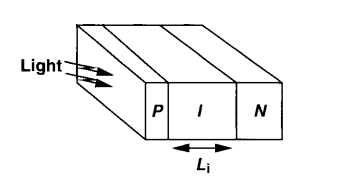
\includegraphics[scale=0.4]{Imagens/PIN.png}
	\end{center}
	\legend{Fonte: \cite{RazaviOpt}}
\end{figure}

Quando um fóton com energia suficiente para excitar o material \'e absorvido, um par el\'etron-lacuna \'e gerado (migração de um el\'etron da banda de valência para de condução), e por difusão, os el\'etrons migram para o cátodo, formando uma fotocorrente. Ajustando-se os tamanhos das camadas P, N e da região de depleção (formada pelo semicondutor intrínseco), podemos controlar a resposta em frequência do fotodiodo e qual a energia mínima do fóton necessária para que gere a fotocorrente. Com a migração dos el\'etrons, uma diferença de potencial \'e gerada entre as camadas P e N, que pode ser aproveitada para a geração de corrente el\'etrica em um circuito el\'etrico fechado \cite{hamamatsu}.
Um fotodiodo apresenta um modelo el\'etrico equivalente ilustrado na \autoref{fig_modelofotodiodo}:

\begin{figure}[htb]
	\caption{\label{fig_modelofotodiodo}Modelo el\'etrico de um fotodiodo}
	\begin{center}
	    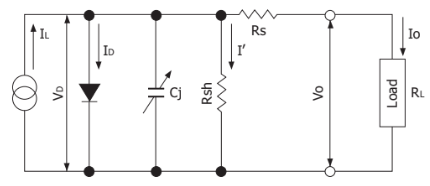
\includegraphics[scale=0.5]{Imagens/ModeloFotodiodo.png}
	\end{center}
	\legend{Fonte: \cite{hamamatsu}}
	\label{modeloElFotodiodo}
\end{figure}

    O modelo el\'etrico apresenta a seguinte express\~ao:

\begin{equation}
    \label{eq_modEletFot}
    I_o = I_L - I_D - I\rq = I_L - I_S*(\exp (\frac{qV_d}{kT})-1) - I\rq
\end{equation}

Onde:
\begin{itemize}
    \item \emph{I\textsubscript{o}} \'e a corrente de saída presente na carga [\emph{A}]
    \item \emph{V\textsubscript{o}} \'e a tensão de saída [\emph{V}]
    \item \emph{R\textsubscript{L}} \'e a carga de saída [\emph{$\Omega$}]
    \item \emph{V\textsubscript{D}} \'e a tens\~ao presente no diodo do modelo el\'etrico equivalente [\emph{V}]
    \item $I_L$ \'e a corrente fotogerada pela fonte luminosa[\emph{A}]
    \item  \emph{I\textsubscript{D}} \'e a corrente corrente de escuro do fotodiodo (sem a presença de luz) [\emph{A}]
    \item \emph{C\textsubscript{j}} \'e a capacit\^ancia de junç\~ao [F]
    \item \emph{R\textsubscript{sh}} \'e a resist\^encia shunt do modelo el\'etrico equivalente [$\Omega$]
    \item \emph{I\rq} \'e a corrente shunt presente na resistência shunt do modelo el\'etrico equivalente [A]
    \item \emph{R\textsubscript{S}} \'e a resistência em s\'erie com a carga de saída do modelo el\'etrico equivalente [$\Omega$]
    \item \emph{q} \'e a carga el\'etrica de um el\'etron [C], \item \emph{k} \'e a constante de Boltzmann [J.K$^{-1}$],
    \item \emph{T} \'e a temperatura presente no fotodiodo [K]
\end{itemize}

O fotodiodo em uma grande faixa apresenta comportamento linear, e \'e a faixa de principal interesse em aplica{\c c}\~oes como o $APS$ ou o $TIA$. Com o aumento do n\'umero de f\'otons recebidos, o n\'ivel de corrente tende a ficar cada vez mais negativo, como mostrado na \autoref{fig_respFotodiodo}. Com o aumento ou diminui{\c c}\~ao expressiva, o circuito come{\c c}a a se tornar n\~ao-linear.

\begin{figure}[htb]
	\caption{\label{fig_respFotodiodo}Resposta Tens\~ao x Corrente para dada intensidade luminosa no fotodiodo}
	\begin{center}
	    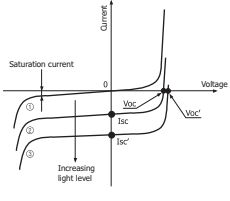
\includegraphics[scale=0.8]{Imagens/graficoRespostaFotodiodo.png}
	\end{center}
	\legend{Fonte: \cite{hamamatsu}}
\end{figure}

\subsection{Figuras de M\'erito}
Do fotodiodo podemos extrair diversas m\'etricas (Figuras de M\'erito), que são de interesse para comparar diferentes modelos. As principais Figuras de M\'erito encontradas na literatura são descritas abaixo, apresentados em \cite{LidianeCampos}.

\subsubsection{Eficiência Quântica}
Relação entre o número de portadores detectados nos terminais das camadas PN do fotodetector, dividido pela incidência de uma determinada quantidade de fótons no fotodetector.

\begin{equation}
    \eta = \frac{N_e}{N_p}
\end{equation}

Onde:
\begin{itemize}
    \item \emph{$\eta$} \'e Efici\^encia Qu\^antica [Adm.]
    \item \emph{N$_e$} \'e o n\'umero de portadores que podem ser detectados nos terminais externos do fotodetector [n° portadores]
    \item \emph{N$_p$} incid\^encia de determinada quantidade de f\'otons [n° f\'otons]
\end{itemize}

\subsubsection{Responsividade}
Razão entre a corrente fotogerada e a potência óptica incidida no fotodiodo.

\begin{equation}
    \label{eq_responsividade}
    R_\lambda = \frac{I_{PH}}{P_{FD}}
\end{equation}

Onde:
\begin{itemize}
    \item \emph{R$_\lambda$} \'e a Responsividade [A.W$^{-1}$]
    \item \emph{I$_{PH}$} \'e a corrente fotogerada [A]
    \item \emph{P$_{FD}$} \'e a pot\^encia \'optica presente no fotodiodo [W]
\end{itemize}

A Eficiência Quântica e a Responsividade se relacionam de acordo com a \autoref{eqEfResp}.

A \autoref{fig_eqEfResp} mostra o gráfico da Responsividade e Efici\^encia Qu\^antica de alguns materiais.

\begin{equation}
    \label{eqEfResp}
    R_\lambda = \frac{\lambda\eta}{1,24}
\end{equation}

Onde:
\begin{itemize}
    \item \emph{R$_\lambda$} \'e a Responsividade [A.W$^{-1}$]
    \item $\lambda$ \'e o comprimento de onda da luz incidente [m]
    \item $\eta$ \'e Efici\^encia Qu\^antica [Adm.]
\end{itemize}

\begin{figure}[htb]
	\caption{\label{fig_responsividade}Responsividade e Efici\^encia Qu\^antica dos materiais Ge, InGaAs, Si}
	\begin{center}
	    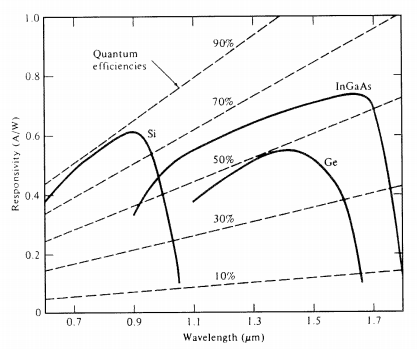
\includegraphics[scale=0.5]{Imagens/GraficoRespostaEspectral.png}
	\end{center}
	\legend{Fonte: \cite{ajoy}}
	\label{fig_eqEfResp}
\end{figure}


\subsubsection{Velocidade de Resposta}
A velocidade de resposta indica o quão rápido o fotodiodo \'e capaz de responder a estímulos de luz externos, em determinada frequência. \'e caracterizado pelo Tempo de Subida e Tempo de Descida do fotodiodo, na faixa de frequências de interesse.

O Tempo de Subida \'e calculado como o tempo do qual um fotodiodo, inicialmente sem incidência de luz, leva para elevar o seu nível em tensão nos seus terminais de 10\% para 90\% do seu pico, a partir do no momento que começar a absorver fótons de uma fonte luminosa controlada, em determinada frequência.

O Tempo de Descida \'e calculado como o tempo do qual um fotodiodo, inicialmente com determinada incidência de luz e já estabilizado na sua respectiva tensão de pico, leva para diminuir a diferença de tensão entre seus terminais de 90\% para 10\% do seu pico, a partir do momento que não absorver mais fótons de origem de uma fonte luminosa controlada, em determinada frequência.

\begin{figure}[htb]
	\caption{\label{fig_velocidadeResp}Representação gr\'afica do Tempo de Subida e Descida}
	\begin{center}
	    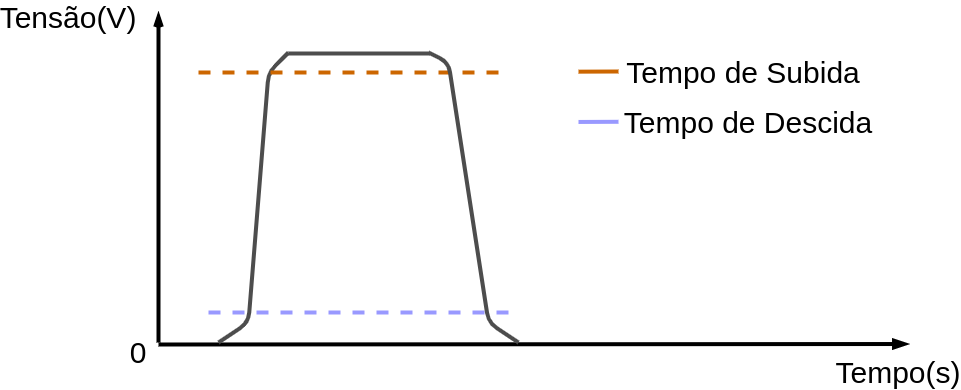
\includegraphics[scale=0.3]{Imagens/GraficoVelocidadeResposta.png}
	\end{center}
	\legend{Fonte: Produzido pelo autor}
\end{figure}

O conhecimento da velocidade de resposta \'e crucial para determinar as limitações do projeto em termos de processamento de informações. A amostragem de dados deve ter período maior do que os tempos de subida e de descida do fotodiodo, nos maiores valores apresentados na faixa de frequência desejada.

\subsubsection{Resposta Espectral}
	O Efeito Fotoel\'etrico se caracteriza pela excitação de el\'etrons em um material por um fóton, quando este apresenta uma energia mínima, chamada de Função Trabalho. Mesmo quando uma grande quantidade de fótons com energia menor do que a Função Trabalho atravessem o fotodiodo, eles não serão capazes de excitar nenhum el\'etron. Como a energia de um fóton diminui com o aumento de seu comprimento de onda, existe um comprimento de onda máximo (ou uma frequência mínima) do qual o fotodetector será capaz de gerar fotocorrente.
	Por outro lado, uma diminuição do comprimento de onda tende a excitar cada vez menos el\'etrons, pois  absorção na região de depleção deixa de acontecer, chegando a um ponto que o fotodiodo sature em resposta e não seja mais possível diferenciar diferentes frequências acima desta.
Sabendo destas limitações, definimos a Resposta Espectral como a faixa de comprimentos de onda do qual o fotodetector \'e capaz de produzir uma fotocorrente correspondente.

\subsubsection{Relação Sinal-Ruído}
Razão entre a potência de sinal fotogerada pela pot\^encia de ru\'ido no sinal.

\begin{equation}
    SNR = \frac{P_{SINAL}}{P_{RUÍDO}}
\end{equation}

Onde:
\begin{itemize}
    \item \emph{SNR} \'e relação sinal-ru\'ido [Adm.]
    \item \emph{P$_{SINAL}$} \'e a pot\^encia do sinal fotogerado [W]
    \item \emph{V\textsubscript{D}} \'e a pot\^encia do ruido do sinal fotogerado [W]
\end{itemize}

\subsubsection{Pot\^encia equivalente ao ru\'ido}
Pot\^encia da luz incidida no fotodiodo, que gera uma potência de sinal equivalente ao de ruído em largura de 1 Hz

\begin{equation}
    NEP = P_{Ru\'ido 1 Hz}
\end{equation}

Onde:
\begin{itemize}
    \item \emph{NEP} \'e a pot\^encia da luz incidida no fotodiodo [W]
    \item \emph{$P_{Ruído 1 Hz}$} \'e a pot\^encia do ruído em largura de 1 Hz
\end{itemize}

\subsubsection{Detectividade espec\'ifica}
Razão entre a raiz quadrada da área fotossensível do diodo, sobre o NEP

\begin{equation}
    D* = \frac{\sqrt{A.B}}{NEP}
\end{equation}

Onde:

\begin{itemize}
    \item \emph{D*} \'e a detectividade espec\'ifica [$cm.\sqrt{Hz}.W^{-1}$]
    \item \emph{A} \'e a \'area da regi\~ao fotossens\'ivel do fotodiodo [cm²]
    \item \emph{A} \'e a largura de banda [Hz]
\end{itemize}

\section{Sensor de Pixel Ativo (APS)}
\label{section:APS}
Um APS \'e um dispositivo do qual se aproveita das características de um fotodiodo para gerar um sinal que pode ser amostrado e então quantificado, de forma a produzir informações referentes à luz incidida no fotodetector.

Dentre as várias possibilidades de produção de um circuito APS, aquele estudado ao longo de todo este trabalho se apresenta na \autoref{fig_APS}.

\begin{figure}[htb]
	\caption{\label{fig_APS}Circuito APS do trabalho}
	\begin{center}
	    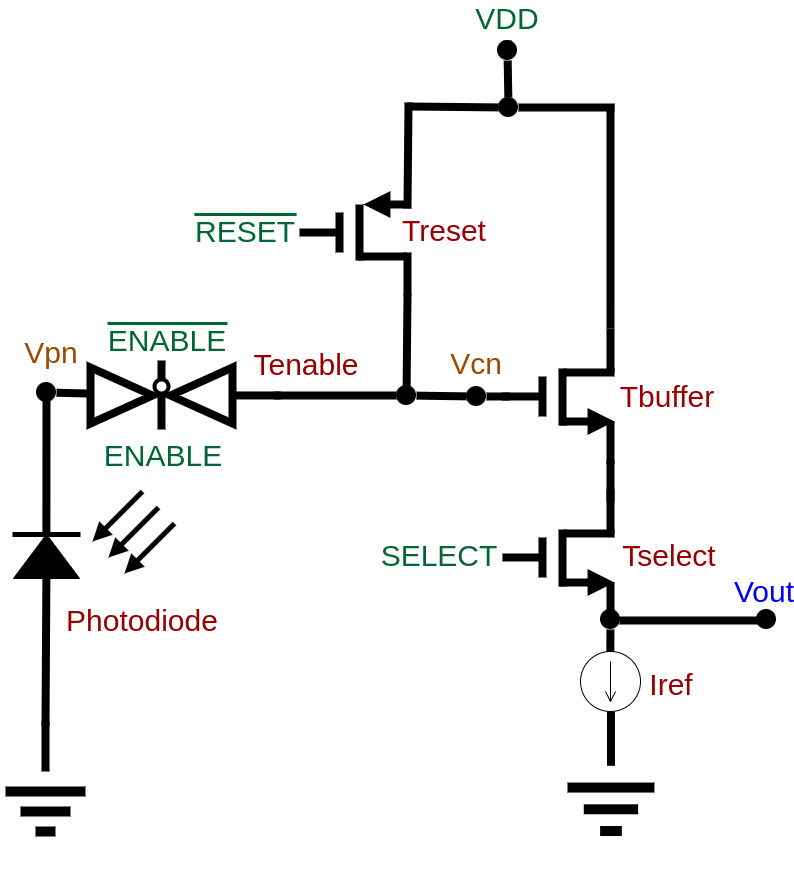
\includegraphics[scale=0.3]{Circuitos/APS.png}
	\end{center}
	\legend{Fonte da ilustra{\c c}\~ao: Pr\'oprio autor}
\end{figure}

\begin{figure}[htb]
	\caption{\label{fig_APS_block}Representa{\c c}\~ao do circuito APS em bloco}
	\begin{center}
	    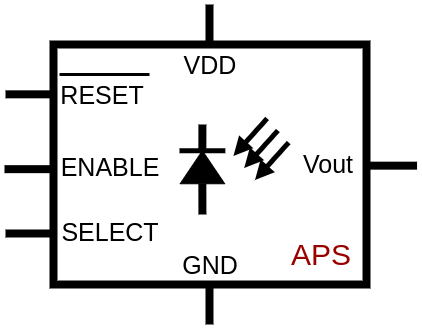
\includegraphics[scale=0.3]{Circuitos/APS_block.png}
	\end{center}
	\legend{Fonte: Produzido pelo autor}
\end{figure}

Cada componente desempenha uma diferente fun{\c c}\~ao de forma a processar a informação advinda da corrente fotogerada:

\begin{itemize}

    \item O transistor \emph{$T_{buffer}$} funciona como um amplificador de Dreno Comum, e seu papel \'e replicar o sinal advindo do n\'o central ao n\'o de sa\'ida, reduzindo o efeito de carga que aconteceria caso o n\'o central ($V_{cn}$) fosse a saída do sistema.

    \item O transistor \emph{$T_{reset}$} funciona como uma chave, que quando fechada (sinal 0 em seu gate), vale \emph{VDD}. Quando aberto (sinal 1 em seu gate), o sinal no n\'o central passa a depender da configuração do transmition gate.

    \item O transmition gate \emph{$T_{enable}$} funciona como uma chave, e quando o transistor \emph{$T_{reset}$} estiver em aberto, tem a função controlar se a tensão presente no fotodiodo ir\'a para o nó central ou n\~ao. Quando aberto, $V_{pn}$ fica isolado do restante do circuito, devido ao estado de alta imped\^ancia nos terminais do dispositivo. Quando fechado, a corrente fotogerada descarrega em $V_{cn}$, pois a associação das capacitâncias parasitas presentes nos transistores de \emph{$T_{enable}$}, \emph{$T_{reset}$} e \emph{$T_{buffer}$} formam um caminho fechado do qual descarrega lentamente o fotodiodo \cite{LidianeCampos}. Uma representa{\c c}\~ao desses capacitores \'e dada na \autoref{fig_APS_cap}.
    
    \item O transistor \emph{$T_{select}$} \'e utilizado para que m\'ultiplos APS's compartilhem um mesmo barramento de sa\'ida. No projeto aqui implementado \emph{$T_{select}$} sempre se apresentar\'a fechado (\emph{SELECT} em n\'ivel l\'ogico '1').
    
    \item A fonte de corrente \emph{$I_{ref}$} tem a fun{\c c}\~ao de polarizar a sa\'ida do circuito, além de aprimorar a linearidade do estágio de sa\'ida \cite{RazaviFundM}.

\end{itemize}

    H\'a dois n\'os internos de bastante interesse ao trabalho, que s\~ao:

\begin{itemize}
    \item \emph{$V_{pn}$}: tens\~ao entre os terminais do fotodiodo
    \item \emph{$V_{cn}$}: tens\~ao no n\'o central do \emph{APS}
\end{itemize}

    Os sinais externos do circuito s\'ao:
    
\begin{itemize}
    \item \emph{RESET}: fecha o transistor \emph{$T_{reset}$}. Ativo em n\'ivel l\'ogico '0'.
     \item \emph{SELECT}: fecha o transistor \emph{$T_{select}$}. Ativo em n\'ivel l\'ogico '1'. No circuito do trabalho estar\'a sempre configurado como '1'.
     \item \emph{ENABLE}: fecha o transmition gate \emph{$T_{enable}$}. Ativo em n\'ivel l\'ogico '1'.
     \item \emph{VDD}: Alimenta{\c c}\~ao do circuito
\end{itemize}

\subsubsection{Capacit\^ancias Parasitas}
Para o correto estudo do \emph{APS} devemos observar as capacit\^ancia equivalente presentes nos n\'os \emph{$V_{pn}$} e \emph{$V_{cn}$} do circuito \cite{LidianeCampos}. Na \autoref{fig_APS_cap} temos uma representa{\c c}\~ao dessas capacit\^ancias.

\begin{figure}[htb]
	\caption{\label{fig_APS_cap}Representa{\c c}\~ao do circuito APS com suas capacit\^ancias parasitas destacadas}
	\begin{center}
	    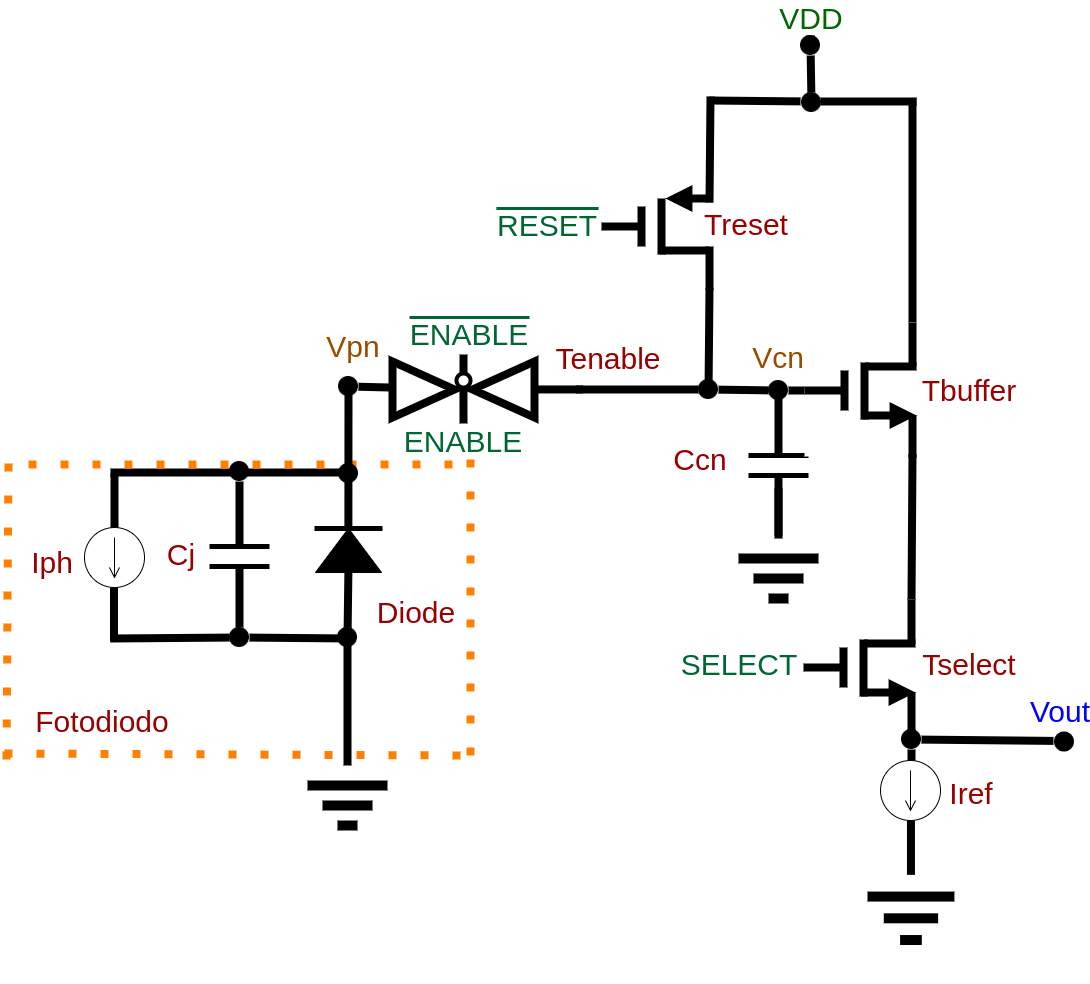
\includegraphics[scale=0.3]{Circuitos/APS_cap.png}
	\end{center}
	\legend{Fonte: Produzido pelo autor}
\end{figure}

\clearpage

Onde: 

\begin{itemize}
    \item $C_j$ \'e a capacit\^ancia de jun{\c c}\~ao do fotodiodo. Seu principal efeito no estudo do APS \'e limitar a velocidade de varia{\c c}\~ao da corrente fotogerada.
    \item $C_{cn}$ \'e a capacit\^ancia equivalente vista do n\'o \emph{$V_{cn}$} ao terra, devido principalmente \'as capacit\^ancias presentes em \emph{$T_{enable}$},  \emph{$T_{reset}$} e \emph{$T_{buffer}$}, sendo o de \emph{$T_{buffer}$} o de maior contribui{\c c}\~ao. O capacitor cria um caminho fechado para a corrente do fotodiodo circular ao terra e ser descarregado em um dos est\'agios citados posteriormente no trabalho.
    \item \emph{$I_{ph}$} \'e a corrente fotogerada
    \item \emph{Diode} \'e o diodo do modelo el\'etrico equivalente do fotodiodo
    \emph{}
\end{itemize}

\subsubsection{Est\'agios}
\label{estagiosAPS}

A operação do APS pode ser dividida em 4 est\'agios, que vão definir os m\'inimos momentos de  atua{\c c}\~ao no sinal de controle e seus limites opera{\c c}\~ao. Os est\'agios s\~ao representados na \autoref{figura_estagiosAPS}, tendo como base o trabalho de \cite{LidianeCampos}.

\begin{figure}[htb]
	\caption{\label{figura_estagiosAPS}Esbo{\c c}o de resposta do APS ao controlar seus sinais de entrada}
	\begin{center}
	    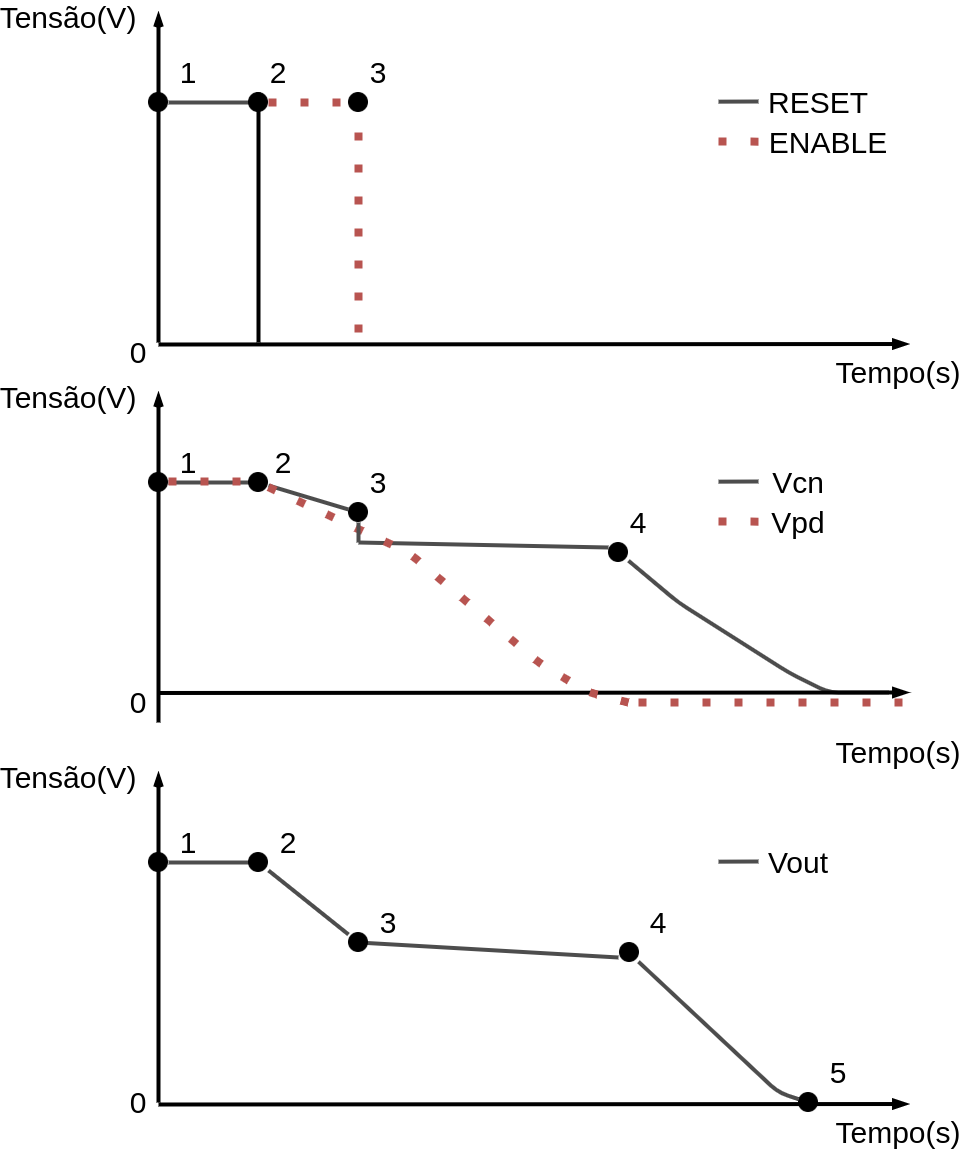
\includegraphics[scale=0.2]{Imagens/estagiosAPS.png}
	\end{center}
	\legend{Fonte: Adaptado de \cite{LidianeCampos}}
\end{figure}

\begin{enumerate}

\item \emph{$T_{reset}$} fechado, \emph{$T_{enable}$} fechado (Período de Reset)
    
Nessa condição, o n\'o $V_{cn}$ \'e igual a VDD.

\item \emph{$T_{reset}$} aberto, \emph{$T_{enable}$} fechado (Período de Integração)

A corrente fotogerada passa a descarregar a capacit\^ancia $C_{cn}$ do nó central, e então pelas capacitância parasita \emph{$C_{cn}$}. A tensão no fotodiodo passa a diminuir, devido a circulação de corrente que diminui a carga de \emph{$C_{j}$}.

A tens\~ao nos terminais do fotodiodo neste segundo est\'agio tem uma rela{\c c}\~ao linear com a corrente fotogerada, conforme descrito na \autoref{eq_modEletFotIl}, que \'e deduzida fazendo an\'alises dos n\'os, desprezando-se a resistência presente em $T_{enable}$ e tamb\^em outra resistências parasitas, como aquelas presentes no modelo elétrico do fotodiodo apresentado na \autoref{modeloElFotodiodo}.

\begin{equation}
    \label{eq_modEletFotIl}
    V(t) = VDD-\frac{I_{PH}}{C_j+C_{cn}}t
\end{equation}

Onde:

\begin{itemize}
    \item $VDD$ \'e a tens\~ao de alimenta{\c c}\~ao do circuito [$V$]
    \item $V$ \'e a tens\~ao presente no terminal de catodo do fotodiodo (\autoref{secao_fotodiodo}) [$V$]
    \item $I_{PH}$ \'e a corrente fotogerada [$A$]
    \item $C_j$ \'e a capacit\^ancia de jun{\c c}\~ao do fotodiodo [$F$]
    \item $C_{cn}$ \'e a capacit\^ancia do n\'o central do APS [$F$]
    \item $t$ \'e o tempo [$s$]
\end{itemize}

\item \emph{$T_{reset}$} aberto, \emph{$T_{enable}$} aberto, potencial \emph{$V_{pd}$} positivo

Logo ap\'os abrir o $T_{enable}$, a fotocorrente n\~ao circula mais no n\'o central, e o fotodiodo continua a ter sua diferen{\c c}a de potencial reduzida, com circula{\c c}\~ao de corrente internamente devido a \emph{$C_j$}. O n\'o central passa a cair bem lentamente devido a correntes de fuga. \emph{$V_{pd}$} cai at\'e chegar a se tornar negativo;

\item \emph{$T_{reset}$} aberto, \emph{$T_{enable}$} aberto, potencial \emph{$V_{pd}$} negativo

Nessa situação, o $T_{enable}$ passa a operar em modo linear. O potencial no n\'o $V_{cn}$ passa a cair devido a circulação de corrente do n\'o at\'e o fotodiodo. O nó diminui at\'e que finalmente chega a 0, onde se mant\'em estável e não apresenta mais circula{\c c}\~ao de corrente.

\end{enumerate}

\subsection{Amostrando informações da luz com um APS básico}
\label{secao_amostrando}

Podemos aproveitar o entendimento das propriedades f\'isicas do fotodiodo, e tamb\'em dos est\'agios de funcionamento de um APS, para obtermos informações relativas aos f\'otons absorvidos.

Como sabemos matematicamente as relações de fotocorrente determinadas por \autoref{eq_modEletFot} e \autoref{eq_modEletFotIl}, e tamb\'em as Figuras de M\'erito que caracterizam o fotodetector, podemos utilizar o APS para coletar as informações em sua sa\'ida e determinar a intensidade da luz

Entre os est\'agios 2 e 3, a tens\~ao do n\'o $V_{cn}$ passa a cair, devido a circula{\c c}\~ao da fotocorrente. Como essa corrente depende da intensidade da luz, podemos descobrir o valor de intensidade sabendo a inclina{\c c}\~ao da curva de tens\~ao na sa\'ida, j\'a que a varia{\c c}\~ao da tens\~ao \'e uma grandeza diretamente proporcional a corrente e a imped\^ancia vista no n\'o. Como a tens\~ao de sa\'ida \'e igual ao de $V_{cn}$ menos $V_{GS}$ do transistor $T_{buffer}$, podemos medir a sa\'ida para processar o sinal e ent\~ao relatar a intensidade luminosa.

Com as observa{\c c}\~oes aqui apresentadas, podemos desenvolver um sistema de medi{\c c}\~ao de informa{\c c}\~ao luminosa, trabalhando entre os est\'agios 1 e 3, e ent\~ao retornando ao 1 para uma nova aquisi{\c c}\~ao. \'E importante destacar que existem limitações quanto \`a temporiza{\c c}\~ao dos est\'agios. Para que a medi{\c c}\~ao seja realizada de forma adequada, devemos garantir que tenhamos entre o Est\'agio 1 e 2, um tempo suficientemente grande para que $V_{cn}$ apresente um valor estável, ou seja, o tempo de transi{\c c}\~ao do sistema nessa condi{\c c}\~ao seja conclu\'ido. Entre o Est\'agio 2 e Est\'agio 3, devemos garantir que tenhamos um tempo mínimo para que dois valores distintos de $V_{out}$ possam ser medidos, de acordo com a sensibilidade do sistema de medi{\c c}\~ao.

\section{Amplificador de Transimped\^ancia (TIA)}
\label{section:TIA}

Um amplificador de transimped\^ancia \'e um circuito em que dada uma corrente de entrada, gera-se uma tens\~ao em sua sa\'ida proporcional \`a esta corrente \cite{RazaviFundM}. Considerando-se o fotodiodo como uma fonte de corrente, a \autoref{fig_TIA} apresenta uma poss\'ivel topologia de um \emph{TIA}, desenvolvido no presente trabalho.

\begin{figure}[htb]
	\caption{\label{fig_TIA}\emph{TIA} desenvolvido}
	\begin{center}
	    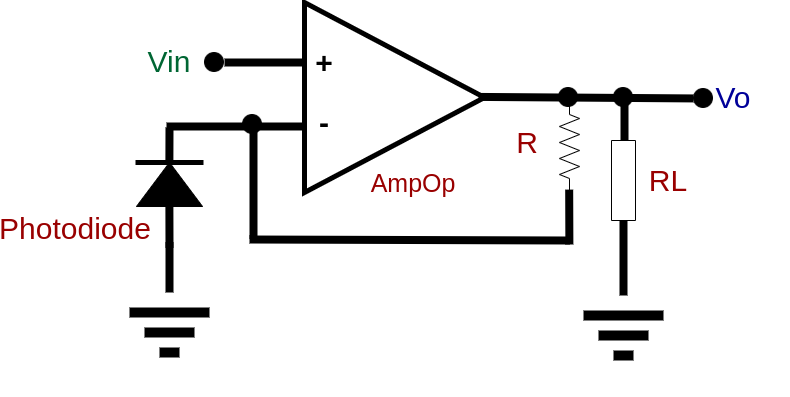
\includegraphics[scale=0.3]{Circuitos/TIA.png}
	\end{center}
	\legend{Fonte da ilustra{\c c}\~ao: Pr\'oprio autor}
\end{figure}

Onde:

\begin{itemize}
    \item $V_{ref}$ \'e a tens\~ao de entrada (ou $referência$) [$V$]
    \item $V_o$ \'e a tens\~ao de sa\'ida [$V$]
    \item $R$ \'e uma resist\^encia de ajuste ganho [$\Omega$]
    \item $R_l$ \'e uma carga de sa\'ida [$\Omega$]
\end{itemize}

Sabemos da \autoref{fig_modelofotodiodo} que podemos modelar uma resist\^encia $R_{sh}$ em paralelo ao fotodiodo. Desprezando-se todos outros componentes do modelo para facilitar a an\'alise, podemos descrever a f\'ormula correspondente ao $TIA$ como a \autoref{eqCTIA}.

\begin{equation}
    \label{eqCTIA}
    V_o = RI_{PH} + (1+\frac{R}{R_{sh}})V_{ref}
\end{equation}

Onde:
\begin{itemize}
    \item $I_{PH}$ \'e a corrente fotogerada [$A$]
\end{itemize}

A \autoref{eqCTIA} nos mostra que \emph{R} deve ser ajustado de forma que n\~ao seja grande demais, pois valores altos (de acordo com a aplicação) irão gerar tens\~ao na sa\'ida com varia{\c c}\~ao muito grande. Mesmo que \emph{Vref} fosse colocado em \emph{GND}, o fator $(1+\frac{R}{R_{sh}})$ ainda pode dominar a relação, devido \'a ruídos presentes no nó, e então impor um termo indesejado, o que também causaria problemas quando \emph{R} fosse muito alto \cite{hamamatsu}.

Devido ao produto $RI_{PH}$, também devemos ter o cuidado de não fazer \textit{R} pequeno demais para que tenhamos a sensibilidade no sinal de saída de forma adequada.

\subsection{Resposta espectral de um \emph{TIA}}

Como a imped\^ancia de entrada do $TIA$ n\~ao \'e ideal (infinita) e varia com a frequ\^encia e temperatura, o circuito n\~ao se apresenta linear em toda sua banda de opera{\c c}\~ao, o que representa uma varia{\c c}\~ao na resposta em frequ\^encia de acordo com a corrente fotogerada \cite{hamamatsu}.
Como o pr\'oprio amplificador apresenta capacit\^ancias internas, o circuito \'e tamb\'em limitado em altas frequ\^encias, principalmente pelo produto $R$ vezes $C$, onde C \'e a capacit\^ancia interna vista pelos terminais de $R$ \cite{hamamatsu}.

Dada as duas propriedades, a \autoref{figura_respostaTIA} e a \autoref{figura_respostaTIA2} mostram o comportamento t\'ipico de resposta em frequ\^encia da topologia.

\begin{figure}[htb]
	\caption{\label{figura_respostaTIA}Resposta espectral de um TIA}
	\begin{center}
	    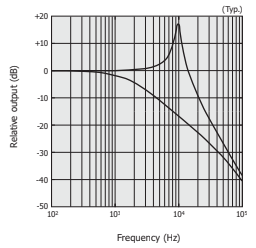
\includegraphics[scale=0.8]{Imagens/RespostaEspectralTIA.png}
	\end{center}
	\legend{Fonte: \cite{hamamatsu}}
\end{figure}

\begin{figure}[htb]
	\caption{\label{figura_respostaTIA2}Resposta a um pulso em um TIA}
	\begin{center}
	    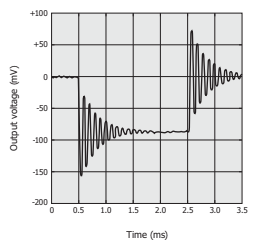
\includegraphics[scale=0.8]{Imagens/RespostaEspectralTIA2.png}
	\end{center}
	\legend{Fonte: \cite{hamamatsu}}
\end{figure}

\clearpage